

\documentclass[24pt,final]{beamer}
\usepackage[scale=1]{beamerposter} % Use the beamerposter package for laying out the poster
\usetheme{confposter} % Use the confposter theme supplied with this template

\setbeamercolor{block title}{fg=ngreen,bg=white} % Colors of the block titles
\setbeamercolor{block body}{fg=black,bg=white} % Colors of the body of blocks
\setbeamercolor{block alerted title}{fg=white,bg=dblue!70} % Colors of the highlighted block titles
\setbeamercolor{block alerted body}{fg=black,bg=dblue!10} % Colors of the body of highlighted blocks
% Many more colors are available for use in beamerthemeconfposter.sty

%---------------------------------------------
% Define the column widths and overall poster size
% To set effective sepwid, onecolwid and twocolwid values, first choose how many columns you want and how much separation you want between columns
% In this template, the separation width chosen is 0.024 of the paper width and a 4-column layout
% onecolwid should therefore be (1-(# of columns+1)*sepwid)/# of columns e.g. (1-(4+1)*0.024)/4 = 0.22
% Set twocolwid to be (2*onecolwid)+sepwid = 0.464
% Set threecolwid to be (3*onecolwid)+2*sepwid = 0.708

\newlength{\sepwid}
\newlength{\onecolwid}
\newlength{\twocolwid}
\newlength{\threecolwid}
\setlength{\paperwidth}{48.6in} % A0 width: 46.8in
\setlength{\paperheight}{33.1in} % A0 height: 33.1in
\setlength{\sepwid}{0.024\paperwidth} % Separation width (white space) between columns
\setlength{\onecolwid}{0.22\paperwidth} % Width of one column
\setlength{\twocolwid}{0.464\paperwidth} % Width of two columns
\setlength{\threecolwid}{0.708\paperwidth} % Width of three columns
\setlength{\topmargin}{-0.5in} % Reduce the top margin size
%-----------------------------------------------------------

\usepackage{graphicx}  % Required for including images

\usepackage{booktabs} % Top and bottom rules for tables

%----------------------------------------------------------------------------------------
%	TITLE SECTION 
%----------------------------------------------------------------------------------------

\title{TEOREMA DE HAHN-BANACH} % Poster title

\author{Lester Armando Vallecillo, lester.vallecillo@unah.hn} % Author(s)
%\email{lester.vallecillo@unah.edu.hn}
\institute{Carrera de Matemáticas, Universidad Nacional Autónoma de Honduras} % Instticas itution(s)

%-----------------------------------------------------------------------------
\begin{document}

\addtobeamertemplate{block end}{}{\vspace*{2ex}} % White space under blocks
\addtobeamertemplate{block alerted end}{}{\vspace*{2ex}} % White space under highlighted (alert) blocks
\setlength{\belowcaptionskip}{2ex} % White space under figures
\setlength\belowdisplayshortskip{2ex} % White space under equations
\begin{frame}[t] % The whole poster is enclosed in one beamer frame
\begin{columns}[t] % The whole poster consists of three major columns
\begin{column}{\sepwid}\end{column} % Empty spacer column
\begin{column}{\onecolwid} % The first column

%	OBJECTIVES
%----------------------------------------------------------------------------------------

\begin{alertblock}{Objetivo}

El propósito de estudio es describir los aspectos teóricos relacionados con Teorema de Hahn-Banach y su aplicación en el análisis funcional, el cual se ilustra en tres versiones diferentes.

\end{alertblock}

%	INTRODUCTION
%--------------------------------------------------------------
\begin{block}{Introducción}
La estructura del análisis funcional tiene como base el estudio de la teoría de dualidad en algunos espacios fundamentales y/o clásicos, de los cuales no se puede asegurar la existencia de funcionales lineales continuos en su dual no nulos, para dotar dichos espacios de propiedades mas generales.\\[0.7cm]

Para garantizar que el dual de un espacio arbitrario sobre un cuerpo de escalares real sea no trivial, se utiliza una de las herramientas pilares del análisis funcional descrita como la versión analítica del teorema de Hahn-Banach. \\[0.7cm]

Una importante aplicación de este resultado es el teorema de extensión de Hahn-Banach en espacios normados, el cual propone extender un funcional lineal definido en un subconjunto de un espacio normado a todo el espacio,  preservando la acotación del funcional definido en todo el espacio normado  \cite{Cabello:2009qr}. \\[0.7cm]

La versión geométrica del teorema  se centra en resumir distintos teoremas de separación de conjuntos convexos como la separación de espacios vectoriales complejos mediante un hiperplano afín. \\[0.7cm]
\end{block}
%------------------------------------------------
\begin{figure}
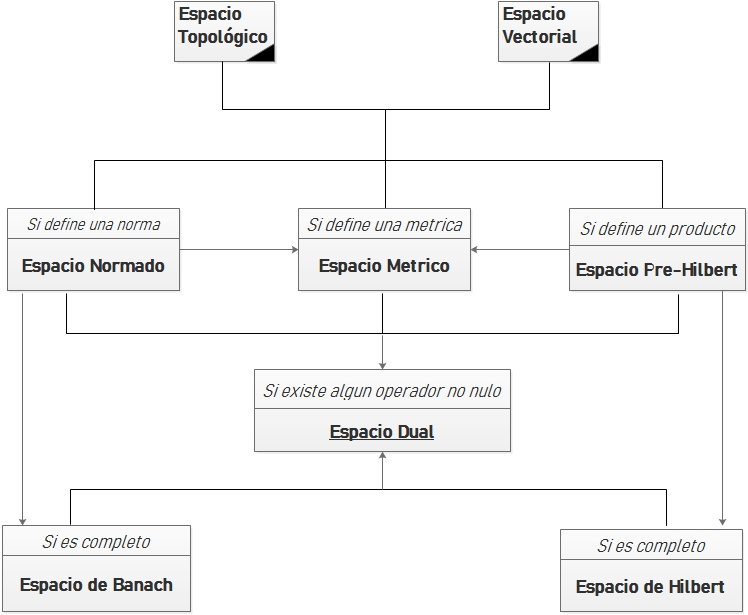
\includegraphics[width=0.98\linewidth]{Pic/ESQUEMA01.jpg}
\caption{Enfoque de la teoría de dualidad sobre espacios fundamentales del análisis funcional. [Fuente: propia] }
\end{figure}


%----------------------------------------------------------------------------------------

\end{column} % End of the first column

\begin{column}{\sepwid}\end{column} % Empty spacer column

\begin{column}{\twocolwid} % Begin a column which is two columns wide (column 2)

\begin{columns}[t,totalwidth=\twocolwid] % Split up the two columns wide column

\begin{column}{\onecolwid}\vspace{-.6in} % The first column within column 2 (column 2.1)

%----------------------------------------------------------------------------------------
%	MATERIALS
%----------------------------------------------------------------------------------------

\begin{block}{Antecedentes}
Helly en 1921 investigó las nociones geométricas ligadas a la convexidad, y su relación con la norma. Con esta idea, logro introducir nuevas técnicas de demostración usando la separabilidad del espacio y el principio de inducción. Estos resultados fueron fundamentales para la solución del problema que obtuvo Hahn.\\[0.7cm]

La versión analítica del Teorema de Hahn-Banach fue demostrada por el matemático austríaco Hahn en 1927 para un espacio normado definido en un cuerpo de escalares real.\\[0.7cm]

Tomando como base el resultado de Hahn,  en 1929 Banach demostró un planteamiento más general,  utilizar funcionales lineales dominados por una seminorma y aplicarlos para obtener resultados de dualidad, esta aplicación es el teorema de extensión \cite{Bombal:2003jr}.\\[0.7cm]

De esta manera, surge la teoría de dualidad como base abstracta del análisis funcional, y en sus aspectos teóricos se destaca el teorema de Hahn-Banach.


\end{block}

%----------------------------------------------------------------------------------------

\end{column} % End of column 2.1

\begin{column}{\onecolwid}\vspace{-.6in} % The second column within column 2 (column 2.2)

%---------------------- ------------------------------------------------------------------
\begin{block}{Aspectos teóricos}
 
\begin{figure}[h]
	\centering
	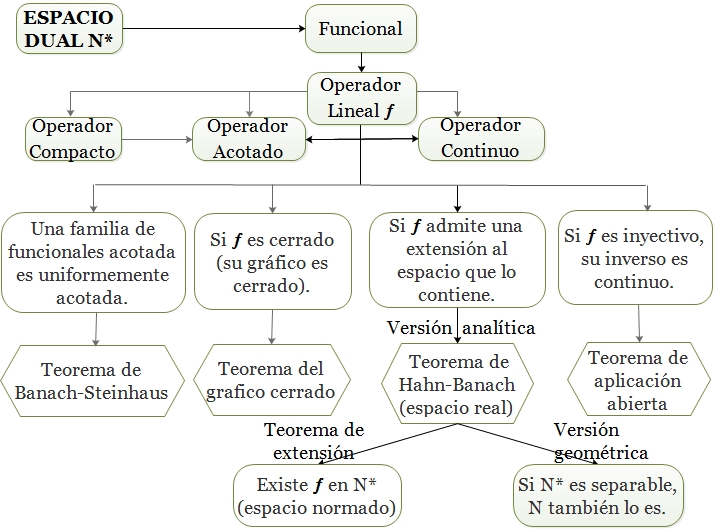
\includegraphics[scale=1.4]{Pic/Esquema02}
	\caption{Enfoque de abstracción de la teoría de dualidad. [Fuente: propia]}\label{02}	
\end{figure}

\end{block}

%----------------------------------------------------------------------------------------

\end{column} % End of column 2.2

\end{columns} % End of the split of column 2 - any content after this will now take up 2 columns width

%----------------------------------------------------------------------------------------
%	IMPORTANT RESULT
%----------------------------------------------------------------------------------------

\begin{alertblock}{Teorema de Hahn-Banach(Versión Analítica)}
Sean $f: \mathbb{V} \longrightarrow \mathbb{R}$ un funcional sobre un espacio vectorial real,  $p \in \mathbb{V}$* una función sublineal, $ \mathbb{S} \subseteq \mathbb{V}$ un subespacio, $\mathbb{S}$* el dual de $\mathbb{S}$, con $f \in \mathbb{S}$* un funcional lineal dominado por $p$ y  que cumple la acotación:
\[f(y) \leq p(y) \hspace*{1cm} \forall y \in \mathbb{S} \]

Entonces existe una funcional $\phi \in \mathbb{V}$*
que cumple las condiciones siguientes:

\begin{tabular}{l  r}
a)	 $ \phi(x) \leq p(x)$ & $ \forall x \in \mathbb{V}$\\
b)	 $\phi$ extiende a $f$, entonces, $\phi(y) = f(y)$ & $\forall y \in \mathbb{S}$.\\[1cm]
\end{tabular} 
\begin{center}

Es decir,   $
\begin{array}[c]{c c c c c c l}%
\phi: & \mathbb{V} & & & \phi \leq p            & & \\
& \mid & \searrow & &                   & \Longrightarrow & \phi(y) = f(y)\\ 
f: & \mathbb{S} & \longrightarrow & \mathbb{R} & f \leq p & & \end{array} $
\end{center}

\end{alertblock} 

%----------------------------------------------------------------------------------------

\begin{columns}[t,totalwidth=\twocolwid] % Split up the two columns wide column again

\begin{column}{\onecolwid} % The first column within column 2 (column 2.1)

%----------------------------------------------------------------------------------------
%	MATHEMATICAL SECTION
%----------------------------------------------------------------------------------------

\begin{block}{Teorema de Extensión de Hahn-Banach}
 Si $X$ es espacio normado sobre $K = \mathbb{R}$ o $\mathbb{C}$ y $f \colon \mathbb{S} \to K $ (es decir, $f \in \mathbb{S}$*) es un funcional lineal continuo, entonces existe un funcional continuo $ \phi \in \mathbb{X}$* que extiende a $ f $, de manera que $\forall x \in X$, se cumple que,\\ \[ \left \Vert \phi(x)  \right \Vert = \left \Vert f(x) \right \Vert \] 
 
 Este resultado propone extender todo funcional lineal continuo definido en un subespacio de un espacio normado a todo el espacio, conservando la norma \cite{Cabello:2009qr}.

\end{block}

%----------------------------------------------------------------------------------------

\end{column} % End of column 2.1

\begin{column}{\onecolwid} % The second column within column 2 (column 2.2)

%----------------------------------------------------------------------------------------
%	RESULTS
%----------------------------------------------------------------------------------------

\begin{block}{Versión Geométrica}
Consiste en un conjunto de teoremas teoremas de separación de conjuntos convexos, aplicando la versión analítica del teorema de Hahn-Banach.\\[0.5cm]

 \textbf{Teorema de Separación.} \\
 Si $\mathbb{V}$ es espacio vectorial complejo, $A$ y $B$ subconjuntos convexos de $\mathbb{V}$, no vacíos y disjuntos. Sea $ x_0 \in A$ tal que $ A-x_0 $ es absorbente. Entonces podemos separar $A$ y $B$, si existe un funcional $f: X \longmapsto \mathbb{K}$ y  un hiperplano de ecuación $f(x) =\alpha $ , con $\alpha \in \mathbb{R} $,  tales que $\forall a \in A$, $\forall b \in B$ y se cumple,
$f(a) \leq \sigma \leq f(b)$
\end{block}

%----------------------------------------------------------------------------------------

\end{column} % End of column 2.2

\end{columns} % End of the split of column 2

\end{column} % End of the second column

\begin{column}{\sepwid}\end{column} % Empty spacer column

\begin{column}{\onecolwid} % The third column


\begin{block}{Aplicación al problema de momentos}
El problema de momentos de Hausdorff puede estar asociado a funciones de densidad de carga de partículas ó de distribuciones de probabilidad, si se toma una sucesión de números reales $\{c_n\}$ en el espacio de probabilidades C[0, 1]. \\[0.5cm]

Para asegurar la existencia de un funcional lineal continuo, se define un funcional  de variación acotada $\varphi$, de manera que, para cada $n \in N$ se cumple,
\[  c_n =  {\int_0}^1 t^n d\varphi(t) \] En este problema se dan las condiciones necesarias y suficientes para que un sistema de infinitas ecuaciones e infinitas incógnitas en un espacio normado tenga solución. Este resultado, es consecuencia del teorema de Hahn-Banach.\\
\end{block}

%----------------------------------------------------------------------------------------
%	CONCLUSION
%----------------------------------------------------------------------------------------

\begin{block}{Conclusiones}
El análisis funcional tiene como base la teoría de la dualidad, es decir, su estudio se centra en la abstracción de funcionales lineales que forman el espacio dual no trivial.\\[0.5cm]

Los operadores lineales del dual se pueden extender con el propósito de dotar de propiedades mas generales a algunos espacios fundamentales.\\[0.5cm]

Se puede resolver sistemas de infinitas ecuaciones lineales utilizando el teorema de Hahn-Banach, un aplicación particular es el problema de momentos.\\[0.5cm]

Se propone estudiar aplicaciones del teorema de Hahn-Banach en la áreas de computación ó mecánica cuántica.


\end{block}

%----------------------------------------------------------------
%	REFERENCES
%----------------------------------------------------------------------------------------

\begin{block}{Referencias}

\nocite{*} % Insert publications even if they are not cited in the poster
\small{\bibliographystyle{unsrt}
\bibliography{sample}\vspace{0.75in}}

\end{block}
\begin{center}
\begin{tabular}{ccc}

\includegraphics[width=0.4\linewidth]{logounah} & \hfill \hspace{3cm} & \includegraphics[width=0.2\linewidth]{Facu.jpg}
\end{tabular}
\end{center}

\end{column} % End of the third column

\end{columns} % End of all the columns in the poster

\end{frame} % End of the enclosing frame

\end{document}
